Hopefully by now you've run Rivet a few times and got the hang of the command
line interface and viewing the resulting analysis data files. Maybe you've got
some ideas of analyses that you would like to see in Rivet's library. If so,
then you'll need to know a little about Rivet's internal workings before you can
start coding: with any luck by the end of this section that won't seem
particularly intimidating.

The core objects in Rivet are ``projections'' and ``analyses''. Hopefully
``analyses'' isn't a surprise --- that's just the collection of routines that
will make histograms to compare with reference data, and the only things that
might differ there from experiences with HZTool\cite{Bromley:1995np} are the new histogramming system
and the fact that we've used some object orientation concepts to make life a bit
easier. The meaning of ``projections'', as applied to event analysis, will
probably be less obvious. We'll discuss them soon, but first a
semi-philosophical aside on the ``right way'' to do physics analyses on and
involving simulated data.


\section{The science and art of physically valid MC analysis}

The world of MC event generators is a wonderfully convenient one for
experimentalists: we are provided with fully exclusive events whose most complex
correlations can be explored and used to optimise analysis algorithms and some
kinds of detector correction effects. It is absolutely true that the majority of
data analyses and detector designs in modern collider physics would be very
different without MC simulation.

But it is very important to remember that it is just simulation: event
generators encode much of known physics and phenomenologically explore the
non-perturbative areas of QCD, but only unadulterated experiment can really tell
us about how the world behaves. The richness and convenience of MC simulation
can be seductive, and it is important that experimental use of MC strives to
understand and minimise systematic biases which may result from use of simulated
data, and to not ``unfold'' imperfect models when measuring the real world. The
canonical example of the latter effect is the unfolding of hadronisation (a
deeply non-perturbative and imperfectly-understood process) at the Tevatron (Run
I), based on MC models. Publishing ``measured quarks'' is not physics --- much
of the data thus published has proven of little use to either theory or
experiment in the following years. In the future we must be alert to such
temptation and avoid such gaffes --- and much more subtle ones.

These concerns on how MC can be abused in treating measured data also apply to
MC validation studies. A key observable in QCD tunings is the \pT of the \PZ
boson, which has no phase space at exactly $\pT = 0$ but a very sharp peak at
$\mathcal{O}(\unit{1-2}{\GeV})$. The exact location of this peak is mostly
sensitive to the width parameter of a nucleon ``intrinsic \pT'' in MC
generators, plus some soft initial state radiation and QED
bremsstrahlung. Unfortunately, all the published Tevatron measurements of this
observable have either ``unfolded'' the QED effects to the ``\PZ \pT'' as
attached to the object in the HepMC/HEPEVT event record with a PDG ID code of
23, or have used MC data to fill regions of phase space where the detector could
not measure. Accordingly, it is very hard to make an accurate and portable MC
analysis to fit this data, without similarly delving into the event record in
search of ``the boson''. While common practice, this approach intrinsically
limits the precision of measured data to the calculational order of the
generator --- often not analytically well-defined. We can do better.

Away from this philosophical propaganda (which nevertheless we hope strikes some
chords in influential places\dots), there are also excellent pragmatic reasons
for MC analyses to avoid treating the MC ``truth'' record as genuine truth. The
key argument is portability: there is no MC generator which is the ideal choice
for all scenarios, and an essential tool for understanding sub-leading
variability in theoretical approaches to various areas of physics is to use
several generators with similar leading accuracies but different sub-leading
formalisms. While the HEPEVT record as written by HERWIG and PYTHIA has become
familiar to many, there are many ambiguities in how it is filled, from the
allowed graph structures to the particle content. Notably, the Sherpa event
generator explicitly elides Feynman diagram propagators from the event record,
perhaps driven by a desire to protect us from our baser analytical
instincts. The Herwig++ event generator takes the almost antipodal approach of
expressing different contributing Feynman diagram topologies in different ways
(\emph{not} physically meaningful!) and seamlessly integrating shower emissions
with the hard process particles. The general trend in MC simulation is to blur
the practically-induced line between the sampled matrix element and the
Markovian parton cascade, challenging many established assumptions about ``how
MC works''. In short, if you want to ``find'' the \PZ to see what its \pT or
$\eta$ spectrum looks like, many new generators may break your honed PYTHIA
code\dots or silently give systematically wrong results. The unfortunate truth
is that most of the event record is intended for generator debugging rather than
physics interpretation.

Fortunately, the situation is not altogether negative: in practice it is usually
as easy to write a highly functional MC analysis using only final state
particles and their physically meaningful on-shell decay parents. These are,
since the release of HepMC 2.5, standardised to have status codes of 1 and 2
respectively. \PZ-finding is then a matter of choosing decay lepton candidates,
windowing their invariant mass around the known \PZ mass, and choosing the best
\PZ candidate: effectively a simplified version of an experimental analysis of
the same quantity. This is a generally good heuristic for a safe MC analysis!
Note that since it's known that you will be running the analysis on signal
events, and there are no detector effects to deal with, almost all the details
that make a real analysis hard can be ignored. The one detail that is worth
including is summing momentum from photons around the charged leptons, before
mass-windowing: this physically corresponds to the indistinguishability of
collinear energy deposits in trackers and calorimeters and would be the ideal
published experimental measurement of Drell-Yan \pT for MC tuning. Note that
similar analyses for \PW bosons have the luxury over a true experiment of being
able to exactly identify the decay neutrino rather than having to mess around
with missing energy. Similarly, detailed unstable hadron (or tau) reconstruction
is unnecessary, due to the presence of these particles in the event record with
status code 2. In short, writing an effective analysis which is automatically
portable between generators is no harder than trying to decipher the variable
structures and multiple particle copies of the debugging-level event
objects. And of course Rivet provides lots of tools to do almost all the
standard fiddly bits for you, so there's no excuse!\\[\lineskip]

\noindent
Good luck, and be careful!

% While the event record "truth" structure may look very
% compellingly like a history of the event processes, it is extremely important to
% understand that this is not the case. For starters, such a picture is not
% quantum mechanically robust: it is impossible to reconcile such a concept of a
% single history with the true picture of contributing and interfering
% amplitudes. A good example of this is in parton showers, where QM interference
% leads to colour coherence. In the HERWIG-type parton showers, this colour
% coherence is implemented as an angular-ordered series of emissions, while in
% PYTHIA-type showers, an angular veto is instead applied. The exact history of
% which particles are emitted in which order is not physically meaningful but
% rather an artefact of the model used by the generator --- and is primarily
% useful for generator authors' debugging rather than physics analysis. This is in
% general true for all particles in the event without status codes of 1, 2 or 4.

% Another problem is that the way in which the event internals is documented is
% not well defined: it is for authors' use and as such they can do anything they
% like with the "non-physics" entities stored within. Some examples:

%     * Sherpa does not write matrix element particles (i.e. W, Z, Higgs, ...) into the event record in most processes
%     * Herwig++ uses very low-mass Ws in its event record to represent very off-shell weak decay currents of B and D mesons (among others)
%     * In Drell-Yan events, Herwig++ sometimes calls the propagating boson a Z, and sometimes a photon, probabilistically depending on the no-mixing admixture terms
%     * Sherpa events (and maybe others) can have "bottleneck" particles through which everything flows. Asking if a particle has e.g. a b-quark (NB. an unphysical degree of freedom!) ancestor might always give the answer "yes", depending on the way that the event graph has been implemented
%     * Different generators do not even use the same status codes for "documentation" event record entries: newer ones tend to represent all internals as generator-specific particles, and emphasise their lack of physical meaning
%     * The generator-level barcodes do not have any reliable meaning: any use of them is based on HEPEVT conventions whihc may break, especially for new generators which have never used HEPEVT
%     * Many (all?) generators contain multiple copies of single internal particles, as a bookkeeping tools for various stages of event processing. Determining which (if any) is physically meaningful (e.g. which boosts were or weren't applied, whether QED radiation was included, etc.) is not defined in a cross-generator way.
%     * The distinction between "matrix element" and "parton shower" is ill-defined: ideally everything would be emitted from the parton shower and indeed the trend is to head at least partially in this direction (cf. CKKW/POWHEG). You probably can't make a physically useful interpretation of the "hard process", even if particular event records allow you to identify such a thing.
%     * Quark and gluon jets aren't as simple as the names imply on the "truth" level: to perform colour neutralisation, jets must include more contributions than a single hard process parton. When you look at event graphs, it becomes hard to define these things on a truth level. Use an observable-based heuristic definition instead.

% Hence, any truth-structure assumptions need to checked and probably modified
% when moving from one generator to another: clearly this can lead to
% prohibitively large maintenance and development hurdles. The best approach,
% whenever possible, is to only use truth information to access the particles
% with status code 1 (and those with status = 2, if decays of physically
% meaningful particles (i.e. hadrons) are being studied. In practice, this
% adds relatively little to most analyses, and the portability of the analyses
% is massively improved, allowing for wider and more reliable physics
% studies. If you need to dig deeper, be very careful!

% A final point of warning, more physical than the technicalities above, is that
% the bosons or similar that are written in the event record are imperfect
% calculational objects, rather than genuine truth. MC techniques are improving
% all the time, and you should be extremely careful if planning to do something
% like "unfolding" of QED radiation or initial state QCD radiation on data, based
% on event record internals: the published end result must be meaningfully
% comparable to future fixed order or N^kLL resummation calculations, particularly
% in precision measurements. If not handled with obsessive care, you may end up
% publishing a measurement of the internals of an MC generator rather than
% physical truth! Again, this is not an absolute prohibition --- there are only
% shades of grey in this area --- but just be very careful and stick to statuses
% 1, 2 and 4 whenever possible.


\section{Projections}

\begin{figure}[p]
  \centering
  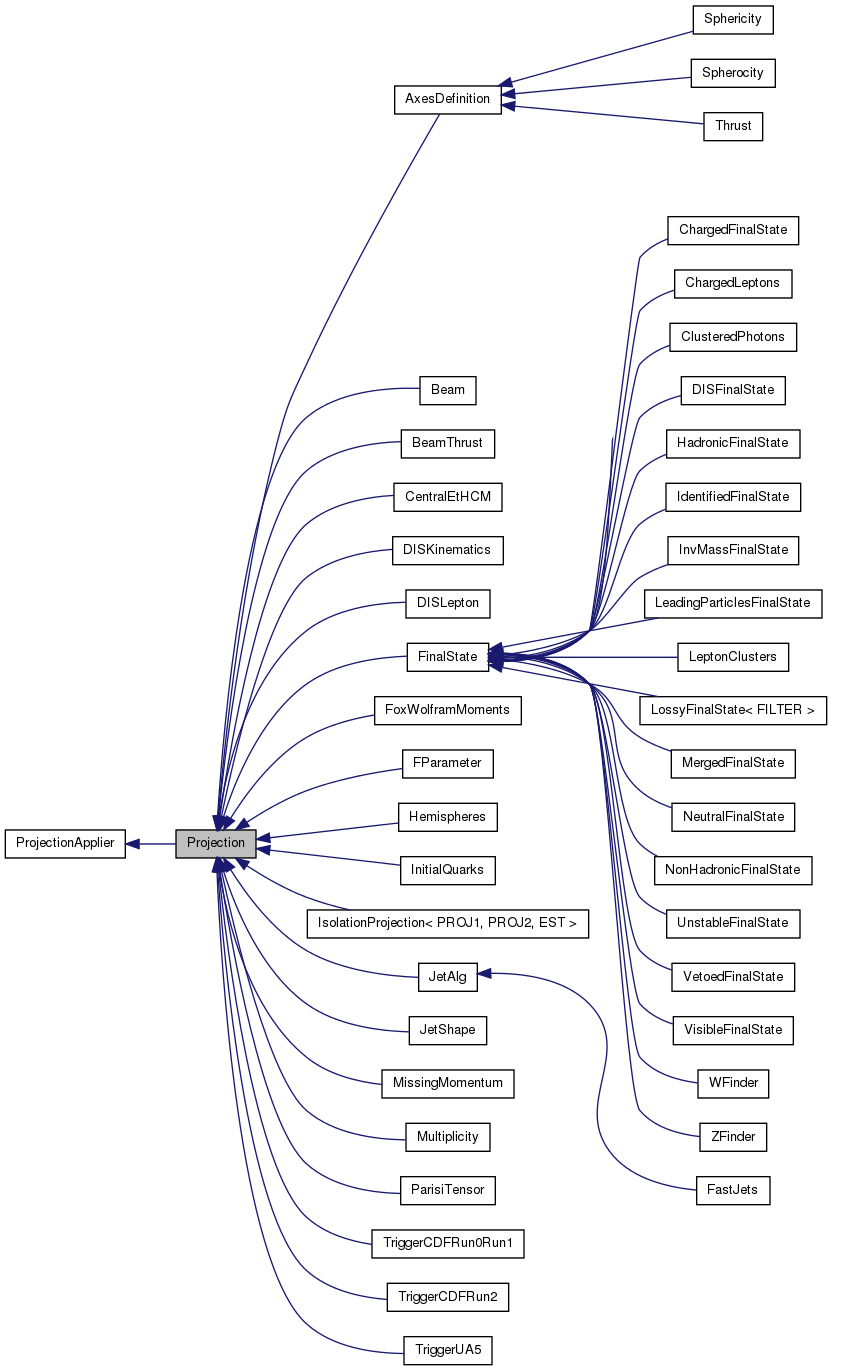
\includegraphics[height=0.98\textheight]{projections.png}
  \caption{List of available projections and their inheritance structure.}
  \label{fig:projections}
\end{figure}

The name ``projection'' is meant to evoke thoughts of projection operators,
low-dimensional slices/views of high-dimensional spaces, and other things that
might appeal to physicists who view the world through quantum-tinted lenses. A
more mundane, but equally applicable, name would be ``observable calculators'',
but since that's a long name, the things they return aren't \emph{necessarily}
observable, and they all inherit from the \kbd{Projection} base class, we'll
stick to that name. It doesn't take long to get used to using the name as a
synonym for ``calculator'', without being intimidated by ideas that they might
be some sort of high-powered deep magic. 90\% of them is simple and
self-explanatory, as a peek under the bonnet of e.g. the all-important
\kbd{FinalState} projection will reveal.

Projections can be relatively simple things like event shapes (i.e. scalar,
vector or tensor quantities), or arbitrarily complex things like lossy or
selective views of the event final state. Most users will see them attached to
analyses by declarations in each analysis' initialisation, but they can also be
recursively ``nested'' inside other projections\footnote{Provided there are no
  dependency loops in the projection chains! Strictly, only acyclic graphs of
  projection dependencies are valid, but there is currently no code in Rivet
  that will attempt to verify this restriction.} (provided there are no infinite
loops in the nesting chain.) Calling a complex projection in an analysis may
actually transparently execute many projections on each event.

You can find a list of all existing projections and their inheritance structure
in Fig.~\ref{fig:projections}. An up-to-date version of this listing can always
be found in the code documentation at \url{http://rivet.hepforge.org}.


\subsection{Projection caching}

Aside from semantic issues of how the class design assigns the process of
analysing events, projections are important computationally because they live in
a framework which automatically stores (``caches'') their results between
events. This is a crucial feature for the long-term scalability of Rivet, as the
previous experience with HZTool was that HERA validation code ran very slowly
due to repeated calculation of the same $k_\perp$ clustering algorithm (at that
time notorious for scaling as the 3rd power of the number of particles.)

A concrete example may help in understanding how this works. Let's say we have
two analyses which have the same run conditions, i.e. incoming beam types, beam
energies, etc. Each also uses the thrust event shape measure to define a set of
basis vectors for their analysis. For each event that gets passed to Rivet,
whichever analysis gets called first will immediately (although maybe
indirectly) call a \kbd{FinalState} projection to get a list of stable, physical
particles (filtering out the intermediate and book-keeping entries in the HepMC
event record). That FS projection is then ``attached'' to the event. Next, the
first analysis will call a \kbd{Thrust} projection which internally uses the
same final state projection to define the momentum vectors used in calculating
the thrust. Once finished, the thrust projection will also be attached to the
event.

So far, projections have offered no benefits. However, when the second analysis
runs it will similarly try to apply its final state and thrust projections to
the event. Rather than repeat the calculations, Rivet's infrastructure will
detect that an equivalent calculation has already been run and will just return
references to the already-run projections. Since projections can also contain
and use other projections, this model allows some substantial computational
savings, without the analysis author even needing to be particularly aware of
what is going on.

Observant readers may have noticed a problem with all this projection caching
cleverness: what if the final states aren't defined the same way? One might
provide charged final state particles only, or the acceptances (defined in
pseudorapidity range and a IR \pT cutoff) might differ. Rivet handles this by
making each projection provide a comparison operator which is used to decide
whether the cached version is acceptable or if the calculation must be re-run
with different settings. Because projections can be nested, applying a top-level
projection to an event can spark off a cascade of comparisons, calculations and
cache accesses, making use of existing results wherever possible.


\subsection{Using projection caching}
So far this is all theory --- how does one actually use projections in Rivet?
First, you should understand that projections, while semantically stored within
each other, are actually all registered with a central \code{ProjectionHandler}
object.\footnote{As of version 1.1 onwards --- previously, they were stored as
  class members inside other \code{Projection}s and \code{Analysis} classes.}
The reason for this central registration is to ensure that all projections'
lifespans are managed in a consistent way, and to protect projection and
analysis authors from some technical subtleties in how C++ polymorphism works.

Inside the constructor of a \code{Projection} or the \code{init} method of an
\code{Analysis} class, you must
call the \code{addProjection} function. This takes two arguments, the projection
to be registered (by \code{const} reference), and a name. The name is local to
the parent object, so you need not worry about name clashes between objects. A
very important point is that the passed \code{Projection} is not the one that is
actually centrally registered --- that distinction belongs to a newly created
heap object which is created within the \code{addProjection} method by means of
the overloaded \code{Projection::clone()} method. Hence it is completely safe
--- and recommended --- to use only local (stack) objects in \code{Projection}
and \code{Analysis} constructors.


\begin{philosophy}
  At this point, if you have rightly bought into C++ ideas like super-strong
  type-safety, this proliferation of dynamic casting may worry you: the compiler
  can't possibly check if a projection of the requested name has been
  registered, nor whether the downcast to the requested concrete type is
  legal. These are very legitimate concerns!

  In truth, we'd like to have this level of extra safety: who wouldn't? But in
  the past, when projections were held as members of \code{ProjectionApplier}
  classes rather than in the central \code{ProjectionHandler} repository, the
  benefits of the strong typing were outweighed by more serious and subtle bugs
  relating to projection lifetime and object ``slicing''. At least when the
  current approach goes wrong it will throw an unmissable \emph{runtime} error
  --- until it's fixed, of course! --- rather than silently do the wrong thing.

  Our problems here are a microcosm of the perpetual language battle between
  strict and dynamic typing, runtime versus compile time errors. In practice,
  this manifests itself as a trade-off between the benefits of static type
  safety and the inconvenience of the type-system gymnastics that it engenders.
  We take some comfort from the number of very good programs have been and are
  still written in dynamically typed, interpreted languages like Python, where
  virtually all error checking (barring first-scan parsing errors) must be done
  at runtime. By pushing \emph{some} checking to the domain of runtime errors,
  Rivet's code is (we believe) in practice safer, and certainly more clear and
  elegant. However, we believe that with runtime checking should come a culture
  of unit testing, which is not yet in place in Rivet.

  As a final thought, one reason for Rivet's internal complexity is that C++ is
  just not a very good language for this sort of thing: we are operating on the
  boundary between event generator codes, number crunching routines (including
  third party libraries like FastJet) and user routines. The former set
  unavoidably require native interfaces and benefit from static typing; the
  latter benefit from interface flexibility, fast prototyping and syntactic
  clarity. Maybe a future version of Rivet will break through the technical
  barriers to a hybrid approach and allow users to run compiled projections from
  interpreted analysis code. For now, however, we hope that our brand of
  ``slightly less safe C++'' will be a pleasant compromise.
\end{philosophy}


% \begin{detail}
% \TODO{How projection caching \emph{really} works}
% (skippable, but useful as a reference)
% \end{detail}

% \subsection{Standard projection summary}
% \TODO{foo}

% \subsection{Example projection}
% \TODO{bar}

% \subsection{Cuts and constraints}
% \TODO{baz}


\section{Analyses}

\subsection{Writing a new analysis}

This section provides a recipe that can be followed to write a new analysis
using the Rivet projections.

Every analysis must inherit from \code{Rivet::Analysis} and, in addition to the
constructor, must implement a minimum of three methods.  Those methods are
\code{init()}, \code{analyze(const Rivet::Event\&)} and \code{finalize()}, which
are called once at the beginning of the analysis, once per event and once at the
end of the analysis respectively.

The new analysis should include the header for the base analysis class plus
whichever Rivet projections are to be used, and should work under the
\code{Rivet} namespace. Since analyses are hardly ever intended to be inherited
from, they are usually implemented within a single \kbd{.cc} file with no
corresponding header. The skeleton of a new analysis named \code{UserAnalysis}
that uses the \code{FinalState} projection might therefore start off looking
like this, in a file named \kbd{UserAnalysis.cc}:
%
\begin{snippet}
#include "Rivet/Analysis.hh"

namespace Rivet {

  class UserAnalysis : public Analysis {
  public:
    UserAnalysis() : Analysis("USERANA") { }
    void init() { ... }
    void analyze(const Event& event) { ... }
    void finalize() { ... }
  };

}
\end{snippet}

The constructor body is usually left empty, as all event loop setup is done in
the \code{init()} method: the one \emph{required} constructor feature is to make
a call to its base \code{Analysis} constructor, passing a string by which the
analysis will \emph{register} itself with the Rivet framework. This name is the
one exposed to a command-line or API user of this analysis: usually it is the
same as the class name, which for official analyses is always in upper case.

\begin{warning}
  Early versions of Rivet required the user to declare allowed beam types,
  energies, whether a cross-section is required, etc. in the analysis
  constructor via methods like \code{setBeams(...)} and
  \code{setNeedsCrossSection(...)}. This information is now \emph{much}
  preferred to be taken from the \kbd{.info} file for the analysis, and
  \emph{must} be done this way in analyses submitted for inclusion in future
  Rivet releases.
\end{warning}

% for the \code{UserAnalysis} may impose certain
% requirements upon the events that the analysis will work with.  A call to the
% \code{setBeams} method declares that the analysis may only be run on events with
% specific types of beam particles, for example adding the line
% %
% \begin{snippet}
%   setBeams(PROTON, PROTON);
% \end{snippet}
% %
% \noindent ensures that the analysis can only be run on events from proton-proton
% collisions.  Other types of beam particles that may be used include
% \code{ANTIPROTON}, \code{ELECTRON}, \code{POSITRON}, \code{MUON} and \code{ALL}.
% The latter of these declares that the analysis is suitable for use with any type
% of collision and is the default.

% Some analyses need to know the interaction cross section that was generated by
% the Monte Carlo generator, typically in order to normalise histograms.
% Depending on the Monte Carlo that is used and its interface to Rivet, the cross
% section may or may not be known.  An analysis can therefore declare at the
% beginning of a run that it will need the cross section information during the
% finalisation stages.  Such a declaration can be used to prevent what would
% otherwise be fruitless analyses from running.  An analysis sets itself as
% requiring the cross section by calling inside the constructor
% %
% \begin{snippet}
%   setNeedsCrossSection(true);
% \end{snippet}
% %
% \noindent In the absence of this call the default is to assume that the analysis
% does not need to know the cross section.

The \code{init()} method for the \code{UserAnalysis} class should add to the analysis all
of the projections that will be used.  Projections can be added to an analysis
with a call to \code{addProjection(Projection, std::string)}, which takes as
argument the projection to be added and a name by which that projection can
later be referenced.  For this example the \code{FinalState} projection is to be
referenced by the string \code{"FS"} to provide access to all of the final state
particles inside a detector pseudorapidity coverage of $\pm 5.0$.  The syntax to
create and add that projection is as follows:
%
\begin{snippet}
init() {
  const FinalState fs(-5.0, 5.0);
  addProjection(fs, "FS");
}
\end{snippet}
%
A second task of the \code{init()} method is the booking of all histograms which
are later to be filled in the analysis code. Information about the histogramming
system can be found in Section~\ref{section:histogramming}.

% It is often the case that an analysis is only appropriate for a limited range of
% Monte Carlo kinematic settings.  For example, an analysis may only be suitable
% if the minimum \pT in the hard scatter is above a certain value.  A mechanism
% exists with the \code{Analysis} object to declare the existence of such a cut.
% However, the relevant information must be made available by the Monte Carlo
% generator and, given the potentially large number of such generator-dependent
% cuts, this information is not currently checked by the AGILe generator
% interface.  Nevertheless, an analysis can add a cut in the constructor with a
% call to \code{addCut(const string\&, const Comparison\&, const double)}, which
% takes as its arguments the name of the cut, the comparison operator and a value
% to compare the cut quantity with.  For example, to add a cut stating that the
% hard scatter \pT must be above \unit{3}{\GeV} one should call

% \begin{snippet}
%   addCut("PT", MORE_EQ, 3.0*GeV);
% \end{snippet}


\subsection{Utility classes}

Rivet provides quite a few object types for physics purposes, such as three- and
four-vectors, matrices and Lorentz boosts, and convenience proxy objects for
e.g. particles and jets. We now briefly summarise the most important features of
some of these objects; more complete interface descriptions can be found in the
generated Doxygen web pages on the Rivet web site, or simply by browsing the
relevant header files.

\subsubsection{\code{FourMomentum}}

The \code{FourMomentum} class is the main physics vector that you will encounter
when writing Rivet analyses. Its functionality and interface are similar to the
CLHEP \code{HepLorentzVector} with which many users will be familiar, but
without some of the historical baggage.

\paragraph{Vector components}%
The \code{FourMomentum} \code{E()}, \code{px()}, \code{py()}, \code{pz()} \&
\code{mass()} methods are (unsurprisingly) accessors for the vector's energy,
momentum components and mass. The \code{vector3()} method returns a spatial
\code{Vector3} object, i.e. the 3 spatial components of the 4-vector.

\paragraph{Useful properties}%
The \code{pT()} and \code{Et()} methods are used to calculate the transverse
momentum and transverse energy. Angular variables are accessed via the
\code{eta()}, \code{phi()} and \code{theta()} for the pseudorapidity, azimuthal
angle and polar angle respectively. More explicitly named versions of these also
exist, named \code{pseudorapidity()}, \code{azimuthalAngle()} and
\code{polarAngle()}. Finally, the true rapidity is accessed via the
\code{rapidity()} method. Many of these functions are also available as external
functions, as are algebraic functions such as \code{cross(vec3a, vec3b)}, which
is perhaps more palatable than \code{vec3a.cross(vec3b)}.

\paragraph{Distances}%
The $\eta$--$\phi$ distance between any two four-vectors (and/or three-vectors)
can be computed using a range of overloaded external functions of the type
\code{deltaR(vec1, vec2)}. Angles between such vectors can be calculated via the
similar \code{angle(vec1, vec2)} functions.

\subsubsection{\code{Particle}}
This class is a wrapper around the HepMC \code{GenParticle}
class. \code{Particle} objects are usually obtained as a vector from the
\code{particles()} method of a \code{FinalState} projection.  Rather than having
to directly use the HepMC objects, and e.g. translate HepMC four-vectors into
the Rivet equivalent, several key properties are accessed directly via the
\code{Particle} interface (and more may be added). The main methods of interest
are \code{momentum()}, which returns a \code{FourMomentum}, and \code{pdgId()},
which returns the PDG particle ID code. The PDG code can be used to access
particle properties by using functions such as \code{PID::isHadron()},
\code{PID::threeCharge()}, etc. (these are defined in
\kbd{Rivet/Tools/ParticleIDMethods.hh}.)

\subsubsection{\code{Jet}}
Jets are obtained from one of the jet accessor methods of a projection that
implements the \code{JetAlg} interface, e.g. \code{FastJets::jetsByPt()} (this
returns the jets sorted by \pT, such that the first element in the vector is the
hardest jet --- usually what you want.) The most useful methods are
\code{particles()}, \code{momenta()}, \code{momentum()} (a representative
\code{FourMomentum}), and some checks on the jet contents such as
\code{containsParticleId(pid)}, \code{containsCharm()} and
\code{containsBottom()}.


\subsubsection{Mathematical utilities}
The \kbd{Rivet/Math/MathUtils.hh} header defines a variety of mathematical
utility functions. These include testing functions such as \code{isZero(a)},
\code{fuzzyEquals(a, b)} and \code{inRange(a, low, high)}, whose purpose is
hopefully self-evident, and angular range-mapping functions such as
\code{mapAngle0To2Pi(a)}, \code{mapAngleMPiToPi(a)}, etc.


\subsection{Histogramming}
\label{section:histogramming}

Rivet's histogramming uses the YODA system, composed of ``analysis object''
classes \code{Histo1D}, \code{Profile1D}, \code{Scatter2D}, and less-used 2D
histograms and profiles, and 1D and 3D scatter plots. These can be created
directly in the analysis code, but to hook fully into the multiple-event-weight
and other machinery in Rivet it's normal to book them through \code{Analysis} class methods, to be called in the \code{init}
step of your analysis routine:
%
\begin{snippet}
  void init() {
    _h_one = bookHisto1D(2, 1, 1);
    _h_two = bookProfile1D(3, 1, 2);
    _h_three = bookHisto1D("d00-x00-y00", logscale(50, 1.0, 100.0));
  }
\end{snippet}
%
Here the first two bookings have a rather cryptic 3-integer sequence as the
first arguments. This is the recommended scheme, which corresponds to the
HepData structure of 1D histograms as a combination of $x$ and $y$ axes in a
dataset $d$, giving names of the form \kbd{d\val{d}-x\val{x}-y\val{y}}. This
auto-booking of histograms saves you from having to copy out reams of bin edges
and values into your code, and makes sure that any data bug-fixes in HepData are
easily propagated to Rivet. The reference data files which are used for these
booking methods are distributed and installed with Rivet, you can find them in
the \kbd{\val{installdir}/share/Rivet} directory of your installation. The third
booking is for a histogram for which there is no such HepData entry: it uses the
usual scheme of specifying the name, number of bins and the min/max $x$-axis
limits manually.

Filling the histograms is done in the \code{MyAnalysis::analyse()}
function. Remember to specify the event weight as you fill:
%
\begin{snippet}
  void analyze(const Event& e) {
    [projections, cuts, etc.]
    ...
    _h_one->fill(pT, event.weight());
    _h_two->fill(pT, Nch, event.weight());
    _h_three->fill(fabs(eta), event.weight());
  }
\end{snippet}

Finally, histogram normalisations, scalings, divisions etc. are done in the
\code{MyAnalysis::\-finalize()} method. For normalisations and scalings you will
find appropriate convenience methods \code{Analysis::normalize(histo, norm)} and
\code{Analysis::scale(histo, scalefactor)}. Many analyses need to be scaled to
the generator cross-section, with the number of event weights to pass cuts being
included in the normalisation factor: for this you will have to track the
passed-cuts weight sum yourself via a member variable, but the analysis class
provides \code{Analysis::crossSection()} and \code{Analysis::sumOfWeights()}
methods to access the pre-cuts cross-section and weight sum respectively.


\subsection{Analysis metadata}

To keep the analysis source code uncluttered, and to allow for iteration of data
plot presentation without re-compilation and/or re-running, Rivet prefers that
analysis metadata is provided via separate files rather than hard-coded into the
analysis library. There are two such files: an \emph{analysis info} file, with
the suffix \kbd{.info}, and a \emph{plot styling} file, with the suffix
\kbd{.plot}.

\subsubsection{Analysis info files}

The analysis info files are in YAML format: a simple data format intended to be
cleaner and more human-readable/writeable than XML. As well as the analysis name
(which must coincide with the filename and the name provided to the
\kbd{Analysis} constructor, this file stores details of the collider,
experiment, date of the analysis, Rivet/data analysis authors and contact email
addresses, one-line and more complete descriptions of the analysis, advice on
how to run it, suggested generator-level cuts, and BibTeX keys and entries for
this user manual. It is also where the validation status of the analysis is declared:

See the standard analyses' info files for guidance on how to populate this
file. Info files are searched for in the paths known to the
\kbd{Rivet::getAnalysisInfoPaths()} function, which many be prepended to using
the \var{RIVET_INFO_PATH} environment variable: the first matching file to be
found will be used.


\subsubsection{Plot styling files}

The \kbd{.plot} files are in the header format for the \kbd{make-plots} plotting
system and are picked up and merged with the plot data by the Rivet
\kbd{compare-histos} script which produces the \kbd{make-plots} input data
files. All the analysis' plots should have a \kbd{BEGIN PLOT ... END PLOT}
section in this file, specifying the title and $x$/$y$-axis labels (the
\kbd{Title}, and \kbd{XLabel}/\kbd{YLabel} directives). In addition, you can use
this file to choose whether the $x$ and/or $y$ axes should be shown with a log
scale (\kbd{LogX}, \kbd{LogY}), to position the legend box to minimise clashes
with the data points and MC lines (\kbd{LegendXPos}, \kbd{LegendYPos}) and any
other valid \kbd{make-plots} directives including special text labels or forced
plot range boundaries. Regular expressions may be used to apply a directive to
all analysis names matching a pattern rather than having to specify the same
directive repeatedly for many plots.

See the standard analyses' plot files and the \kbd{make-plots} documentation
(e.g. on the Rivet website) for guidance on how to write these files. Plot info
files are searched for in the paths known to the
\kbd{Rivet::getAnalysisPlotPaths()} function, which many be prepended to using
the \var{RIVET_PLOT_PATH} environment variable. As usual, the first matching
file to be found will be used.



\subsection{Pluggable analyses}

Rivet's standard analyses are not actually built into the main \kbd{libRivet}
library: they are loaded dynamically at runtime as an analysis \emph{plugin
  library}. While you don't need to worry too much about the technicalities of
this, it does mean that you can similarly write analyses of your own, compile
them into a similar plugin library and run them from \kbd{rivet} without ever
having to modify any of the main Rivet sources or build system. This means that
you can write and run your own analyses with a system-installed copy of Rivet,
and not have to re-patch the main library when a newer version comes out
(although chances are you will have to recompile, since the binary interface usually
change between releases.)

To get started writing your analysis and understand the plugin system better,
you should check out the documentation in the wiki on the Rivet website:
\url{http://rivet.hepforge.org/trac/wiki/}. The standard
\kbd{rivet-mkanalysis} and \kbd{rivet-buildplugin} scripts can respectively be
used to make an analysis template with many ``boilerplate'' details filled in
(including bibliographic information from Inspire if available), and to build a
plugin library with the appropriate compiler options.


\subsubsection{Plugin paths}

To load pluggable analyses you will need to set the \var{RIVET_ANALYSIS_PATH}
environment variable: this is a standard colon-separated UNIX path, specifying
directories in which analysis plugin libraries may be found. If it is
unspecified, the Rivet loader system will assume that the only entry is the
\kbd{lib} directory in the Rivet installation area. Specifying the variable adds
new paths for searching \emph{before} the standard library area, and they will
be searched in the left-to-right order in the path variable.

If analyses with duplicate names are found, a warning message is issued and the
first version to have been found will be used. This allows you to override
standard analyses with same-named variants of your own, provided they are loaded
from different directories.

\begin{change}
  In Rivet 2.1.0 and later, this \var{RIVET_ANALYSIS_PATH} variable (and the
  others described below) have an special extra syntax feature: if the
  environment variable ends with a double separator, i.e. \kbd{::}, then the
  default path will not be appended at all. This can be useful if you want to
  make absolutely certain not to fall back to the default locations, for example
  to avoid the ``duplicate analysis'' warnings if you are getting a lot of them.
\end{change}

Several further environment variables are used to load analysis reference data
and metadata files:
\begin{description}
\item[\var{RIVET_REF_PATH}:] A standard colon-separated path list, whose
  elements are searched in order for reference histogram files. If the required
  file is not found in this path, Rivet will fall back to looking in the
  analysis library paths (for convenience, as it is normal for plugin analysis
  developers to put analysis library and data files in the same directory and it
  would be annoying to have to set several variables to make this work), and
  then the standard Rivet installation data directory.
\item[\var{RIVET_INFO_PATH}:] The path list searched first for analysis
  \kbd{.info} metadata files. The search fallback mechanism works as for
  \var{RIVET_REF_PATH}.
\item[\var{RIVET_PLOT_PATH}:] The path list searched first for analysis
  \kbd{.plot} presentation style files. The search fallbacks again work as for
  \var{RIVET_REF_PATH}.
\end{description}
%

These paths can be accessed from the API using the
\kbd{Rivet::getAnalysisLibPaths()} etc. functions, and can be searched for files
using the Rivet lookup rules via the
\kbd{Rivet::find\-Analysis\-LibFile(filename)} etc. functions. See the Doxygen
documentation for more details. In the lookups using these paths, if the
variable ends with a double separator, i.e. \kbd{::}, then the default path will
not be appended: this may be useful in some situations. These functions are also
available in the Python \kbd{rivet} module, with the same behaviours.



\section{Using Rivet as a library}

You don't have to use Rivet via the provided command-line programmes: for some
applications you may want to have more direct control of how Rivet processes
events. Here are some possible reasons:
%
\begin{itemize}
\item You need to not waste CPU cycles and I/O resources on rendering HepMC
  events to a string representation which is immediately read back in. The FIFO
  idiom (Section~\ref{sec:fifo-idiom}) is not perfect: we use it in circumstances
  where the convenience and decoupling outweighs the CPU cost.
\item You don't want to write out histograms to file, preferring to use them as
  code objects. Perhaps for applications which want to manipulate histogram data
  periodically before the end of the run.
\item You enjoy tormenting Rivet developers who know their API is far from
  perfect, by complaining if it changes!
\item \dots and many more!
\end{itemize}

The Rivet API (application programming interface) has been designed in the hope
of very simple integration into other applications: all you have to do is create
a \code{Rivet::Analysis\-Handler} object, tell it which analyses to apply on the
events, and then call its \code{analyse(evt)} method for each HepMC event --
wherever they come from. The API is (we hope) stable, with the exception of the
histogramming parts.

\begin{warning}
  The histogramming interfaces in Rivet have long been advertised as marked for
  replacement, and while progress in that area has lagger far behind our
  ambitions, it \emph{will} happen with the 2.0.0 release, with unavoidable
  impact on the related parts of the API. You have been warned!
\end{warning}

The API is available for C++ and, in a more restricted form, Python. We will
explain the C++ version here; if you wish to operate Rivet (or e.g. use its
path-searching capabilities to find Rivet-related files in the standard way)
from Python then take a look inside the \kbd{rivet} and \kbd{rivet-*} Python
scripts (e.g. \kbd{less `which rivet`}) or use the module documentation cf.
%
\begin{snippet}
> python
>>> import rivet
>>> help(rivet)
\end{snippet}

And now the C++ API. The best way to explain is, of course, by example. Here is
a simple C++ example based on the \kbd{test/testApi.cc} source which we use in
development to ensure continuing API functionality:
%
\begin{snippet}
#include "Rivet/AnalysisHandler.hh"
#include "HepMC/GenEvent.h"
#include "HepMC/IO_GenEvent.h"

using namespace std;

int main() {

  // Create analysis handler
  Rivet::AnalysisHandler rivet;

  // Specify the analyses to be used
  rivet.addAnalysis("D0_2008_S7554427");
  vector<string> moreanalyses(1, "D0_2007_S7075677");
  rivet.addAnalyses(moreanalyses);

  // The usual mess of reading from a HepMC file!
  std::istream* file = new std::fstream("testApi.hepmc", std::ios::in);
  HepMC::IO_GenEvent hepmcio(*file);
  HepMC::GenEvent* evt = hepmcio.read_next_event();
  double sum_of_weights = 0.0;
  while (evt) {
    // Analyse the current event
    rivet.analyze(*evt);
    sum_of_weights += evt->weights()[0];

    // Clean up and get next event
    delete evt; evt = 0;
    hepmcio >> evt;
  }
  delete file; file = 0;

  rivet.setCrossSection(1.0);
  rivet.setSumOfWeights(sum_of_weights); // not necessary, but allowed
  rivet.finalize();
  rivet.writeData("out");

  return 0;
}
\end{snippet}

Compilation of this, if placed in a file called \kbd{myrivet.cc}, into an
executable called \kbd{myrivet} is simplest and most robust with use of the
\kbd{rivet-config} script:
%
\begin{snippet}
g++ myrivet.cc -o myrivet `rivet-config --cppflags --ldflags --libs`
\end{snippet}
%
It \emph{should} just work!

If you are doing something a bit more advanced, for example using the AGILe
package's similar API to generate Fortran generator Pythia events and pass them
directly to the Rivet analysis handler, you will need to also add the various
compiler and linker flags for the extra libraries, e.g.
%
\begin{snippet}
g++ myrivet.cc -o myrivet \
  `rivet-config --cppflags --ldflags --libs` \
  `agile-config --cppflags --ldflags --libs`
\end{snippet}
%
would be needed to compile the following AGILe+Rivet code:
%
\goodbreak
\begin{snippet}
#include "AGILe/Loader.hh"
#include "AGILe/Generator.hh"
#include "Rivet/AnalysisHandler.hh"
#include "HepMC/GenEvent.h"
#include "HepMC/IO_GenEvent.h"

using namespace std;

int main() {
  // Have a look what generators are available
  AGILe::Loader::initialize();
  const vector<string> gens = AGILe::Loader::getAvailableGens();
  foreach (const string& gen, gens) {
    cout << gen << endl;
  }

  // Load libraries for a specific generator and instantiate it
  AGILe::Loader::loadGenLibs("Pythia6:425");
  AGILe::Generator* generator = AGILe::Loader::createGen();
  cout << "Running " << generator->getName()
       << " version " << generator->getVersion() << endl;

  // Set generator initial state for LEP
  const int particle1 = AGILe::ELECTRON;
  const int particle2 = AGILe::POSITRON;
  const double sqrts = 91;
  generator->setInitialState(particle1, energy1, sqrts/2.0, sqrts/2.0);
  generator->setSeed(14283);

  // Set some parameters
  generator->setParam("MSTP(5)", "320"); //< PYTHIA tune
  // ...

  // Set up Rivet with a LEP analysis
  Rivet::AnalysisHandler rivet;
  rivet.addAnalysis("DELPHI_1996_S3430090");

  // Run events
  const int EVTMAX = 10000;
  HepMC::GenEvent evt;
  for (int i = 0; i < EVTMAX; ++i) {
    generator->makeEvent(evt);
    rivet.analyze(evt);
  }

  // Finalize Rivet and generator
  rivet.finalize();
  rivet.writeData("out.yoda");
  generator->finalize();

  return 0;
}
\end{snippet}


% \cleardoublepage
% \part{How Rivet \emph{really} works}
% \label{part:internals}
%
% In time this will be the place to look for all the nitty gritty on what Rivet is
% doing internally. Not very many people need to know that, and the few that do
% currently don't need a manual for it!
%
% \section{Projection caching}
% \TODO{TODO}
%
% \subsection{Writing a Projection comparison operator}
% \TODO{TODO}
